\documentclass[12pt]{article}
\usepackage{tikz}
\usepackage{pgfplots}
\pgfplotsset{compat=1.13}

\usepackage{extsizes}
\usepackage{caption}
\usepackage{multirow}
\usepackage{wrapfig}

\renewcommand{\epsilon}{\ensuremath{\varepsilon}}
\renewcommand{\phi}{\ensuremath{\varphi}}
\renewcommand{\kappa}{\ensuremath{\varkappa}}
\renewcommand{\le}{\ensuremath{\leqslant}}
\renewcommand{\leq}{\ensuremath{\leqslant}}
\renewcommand{\ge}{\ensuremath{\geqslant}}
\renewcommand{\geq}{\ensuremath{\geqslant}}
\renewcommand{\emptyset}{\varnothing}

\newcommand{\lw}{\linewidth}
\usepackage{geometry} % Простой способ задавать поля
\geometry{top=10mm}
\geometry{bottom=30mm}
\geometry{left=25mm}
\geometry{right=20mm}

\usepackage[T2A]{fontenc}			% кодировка
\usepackage[utf8]{inputenc}	
\usepackage[english,russian]{babel}   %% загружает пакет многоязыковой вёрстки
\usepackage{indentfirst}
\usepackage{subfigure}
\usepackage{amsmath,amsfonts,amssymb,amsthm,mathtools} 
\usepackage{graphicx}
\graphicspath{{img/}}
\usepackage{pdfpages}
\usepackage{iunits}
\newcommand\tab[1][0.8cm]{\hspace*{#1}}
\begin{document}
\begin{minipage}{0.6\linewidth}
	Работу выполнили\\
	Самохин Валентин,
	Агафонов Артем, \\
	Степанов Григорий, Кандинский Василий \\ 676 гр.\\[2mm]
	под руководством\\
	Почернина И.\,Г\,.
\end{minipage}
\hfill
\begin{minipage}{0.3\linewidth}\flushright
	Маршрут~IV \ №~2\\[3mm]
	17~сентября 2018~г.,\\
\end{minipage}

\vspace{8mm}
\begin{center}
	\textbf{\Large Лабораторная работа №~5.1.2:}\\[\parskip]
	\LARGE Эффект Комптона
\end{center}
\vspace{0mm}

\paragraph{Цель работы:} С помощью сцинтилляционного спектрометра исследуется энергетический спектр $\gamma$-квантов, рассеянных на графите. Определяется энергия рассеянных $\gamma$-квантов в зависимости от угла рассеяния, а также энергия покоя частиц, на которых происходит комптоновское рассеяние.

\subsection*{Теоретическая справка}
Будем считать, что $\gamma$-излучение~---~поток квантов с энергией $\hbar\omega$ и импульсом $p=\frac{\hbar\omega}{c}$. Эффект Комптона~---~увеличение длины волны рассеянного излучения по сравнению с падающим~---~как результат упругого соударения  $\gamma$-кванта и свободного электрона.
	
Пусть до соударения электрон покоился ($mc^2$), а  $\gamma$-квант имел энергию~$\hbar\omega$ и импульс~$p=~\frac{\hbar\omega}{c}$.

Тогда после соударения:
\[ E_\text{электрона}=\gamma mc^2 \]
\[ p_\text{электрона}=\gamma mv \]
\[ \gamma=\sqrt{\dfrac{1}{1-\frac{v^2}{c^2}}}, \]
а  $\gamma$-квант рассеивается на угол~$\theta$ по отношению к начальному движению:

\begin{figure}[h] 
\begin{minipage}[h]{0.48 \lw}
    \centering
    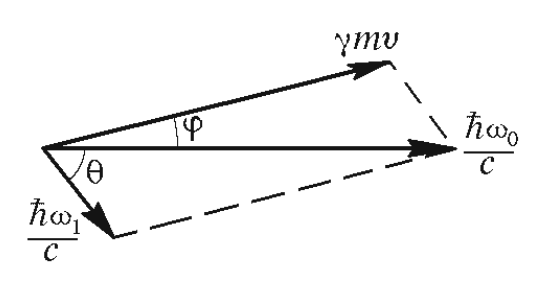
\includegraphics[width=0.8\linewidth]{01}
    \caption{Векторная диаграмма рассеяния}
\end{minipage}
\hfill
\begin{minipage}[h]{0.48 \lw}
\begin{align}
    &E_\gamma = \hbar\omega_1 \\
    &p_\gamma = \frac{\hbar\omega_1}{c} \\
    \text{ЗСЭ: }& mc^2+\hbar \omega_0 = \gamma mc^2+\hbar \omega_1 \\
    \text{ЗСИ: }& \frac{\hbar\omega_0}{c} = \frac{\hbar\omega_1\cos\theta}{c}+\gamma mvcos\varphi \\
    &\gamma mvsin\varphi = \frac{\hbar\omega_1}{c}sin\theta
\end{align}     
\end{minipage}
\end{figure}

Переходя от $\omega_0$, $\omega_1$ к $\lambda_0$, $\lambda_1$:

\begin{equation}
\Delta\lambda=\lambda_1-\lambda_0=\dfrac{h}{mc}(1-\cos\theta)=\Lambda_k(1-\cos\theta)
\label{eq:goal}
\end{equation}
	
$\Lambda_k = \dfrac{h}{mc} = 2.42\cdot 10^{-10}$ \cm~---~комптоновская $\lambda$ электрона.

При рассеянии квантов невысокой ($ 1 \div 10 \K \eV$) энергии часть электронов ведёт себя как связанные, а часть~---~как свободные, т.е. одновременно наблюдаются релеевское и комптоновское рассеяния.
		
Цель работы~---~проверка соотношения \eqref{eq:goal}. Его можно преобразовать от длин волн к энергии квантов:
\[\frac{1}{\varepsilon(\theta)}-\frac{1}{\varepsilon_0}=1-\cos\theta, \quad \varepsilon_0=\frac{E_0}{mc^2} \]

\subsection*{Экспериментальная установка}

\begin{minipage}{0.45\linewidth}[h]
\centering
    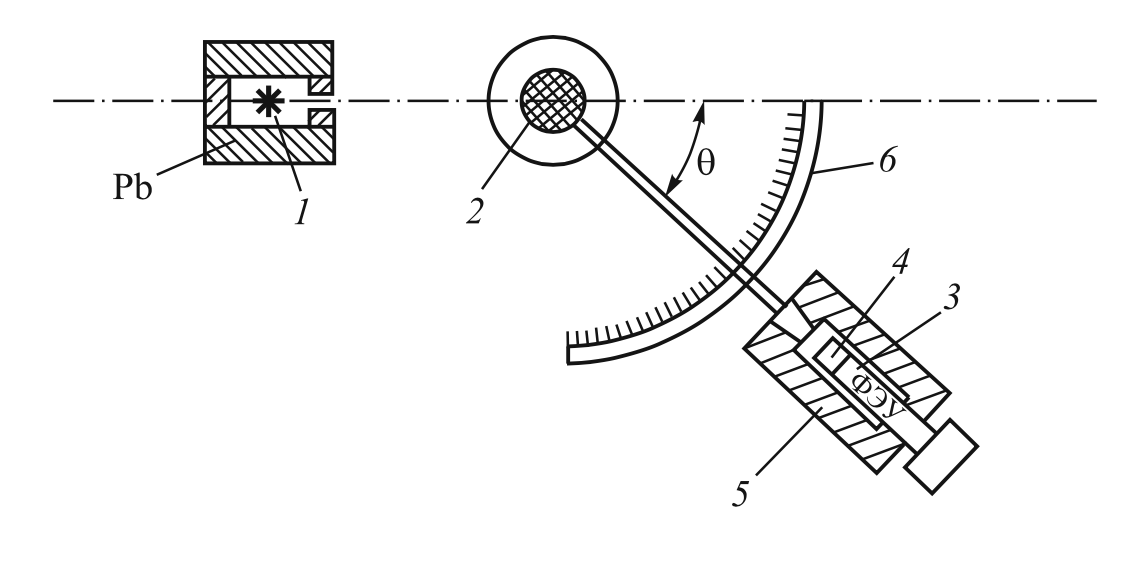
\includegraphics[width=\linewidth]{02}
\captionof{figure}{Блок~-~схема установки по изучению рассеяния $\gamma$-квантов: 1~-~источник излучения ($^{137}Cs$), 2~-~графитовая мишень, 3~-~фотоэлектронный умножитель (ФЭУ), 4~-~сцинтиллятор, 5~-~свинцовый коллиматор, 6~-~лимб}
\end{minipage}
\hfil
\begin{minipage}{0.45\linewidth}[h]
\centering
    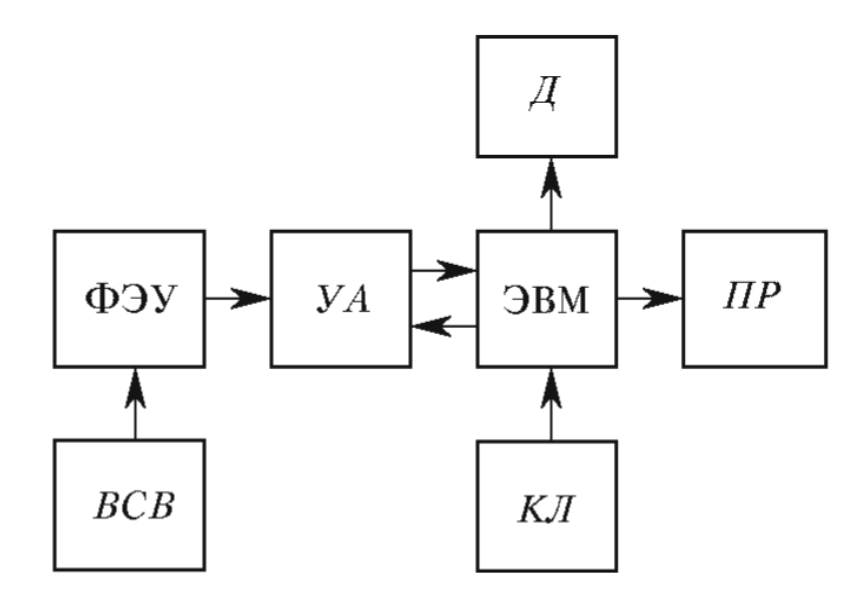
\includegraphics[width=\linewidth]{03}
\captionof{figure}{Блок~-~схема измерительного комплекса: Д~-~дисплей, ПР~-~принтер, ВСВ~-~высоковольтный выпрямитель, УА~-~усилитель~-~анализатор, КЛ~-~клавиатура}
\end{minipage}

%Источник излучения испускает $\gamma$-лучи с энергией 662 кэВ. Кванты, испытавшие комптоновское рассеяние в мишени, регистрируются сцентилляционным счётчиком.

\subsection*{Ход работы}
	Устанавливая сцинтилляционный счётчик под разными углами $\theta$ к первоначальному направлению полёта $\gamma$-квантов, сняли амплитудные спектры и определили положение фотопиков для каждого угла.
	
\begin{table}[h]
\centering
\caption{Результаты измерений:}
\begin{tabular}{|l|c|c|c|c|c|c|c|c|c|c|c|c|c|}
\hline
Угол, $^\circ$ &0 & 10 & 20 & 30 & 40 & 50 & 60 & 70& 80& 90 &100& 110 &120\\ \hline
Канал & 835 & 812& 744 & 701 & 650 & 574 & 500 & 482 & 418 & 368 & 348 & 311 & 258 \\ \hline
\end{tabular}
\end{table}		
\section*{Обработка данных}

\begin{enumerate}
	\item Построили график зависимости $\dfrac{1}{N(\theta)}$ от $(1-\cos\theta)$ и провели через точки наилучшую прямую:			
    \begin{figure} [h]
    	\centering
        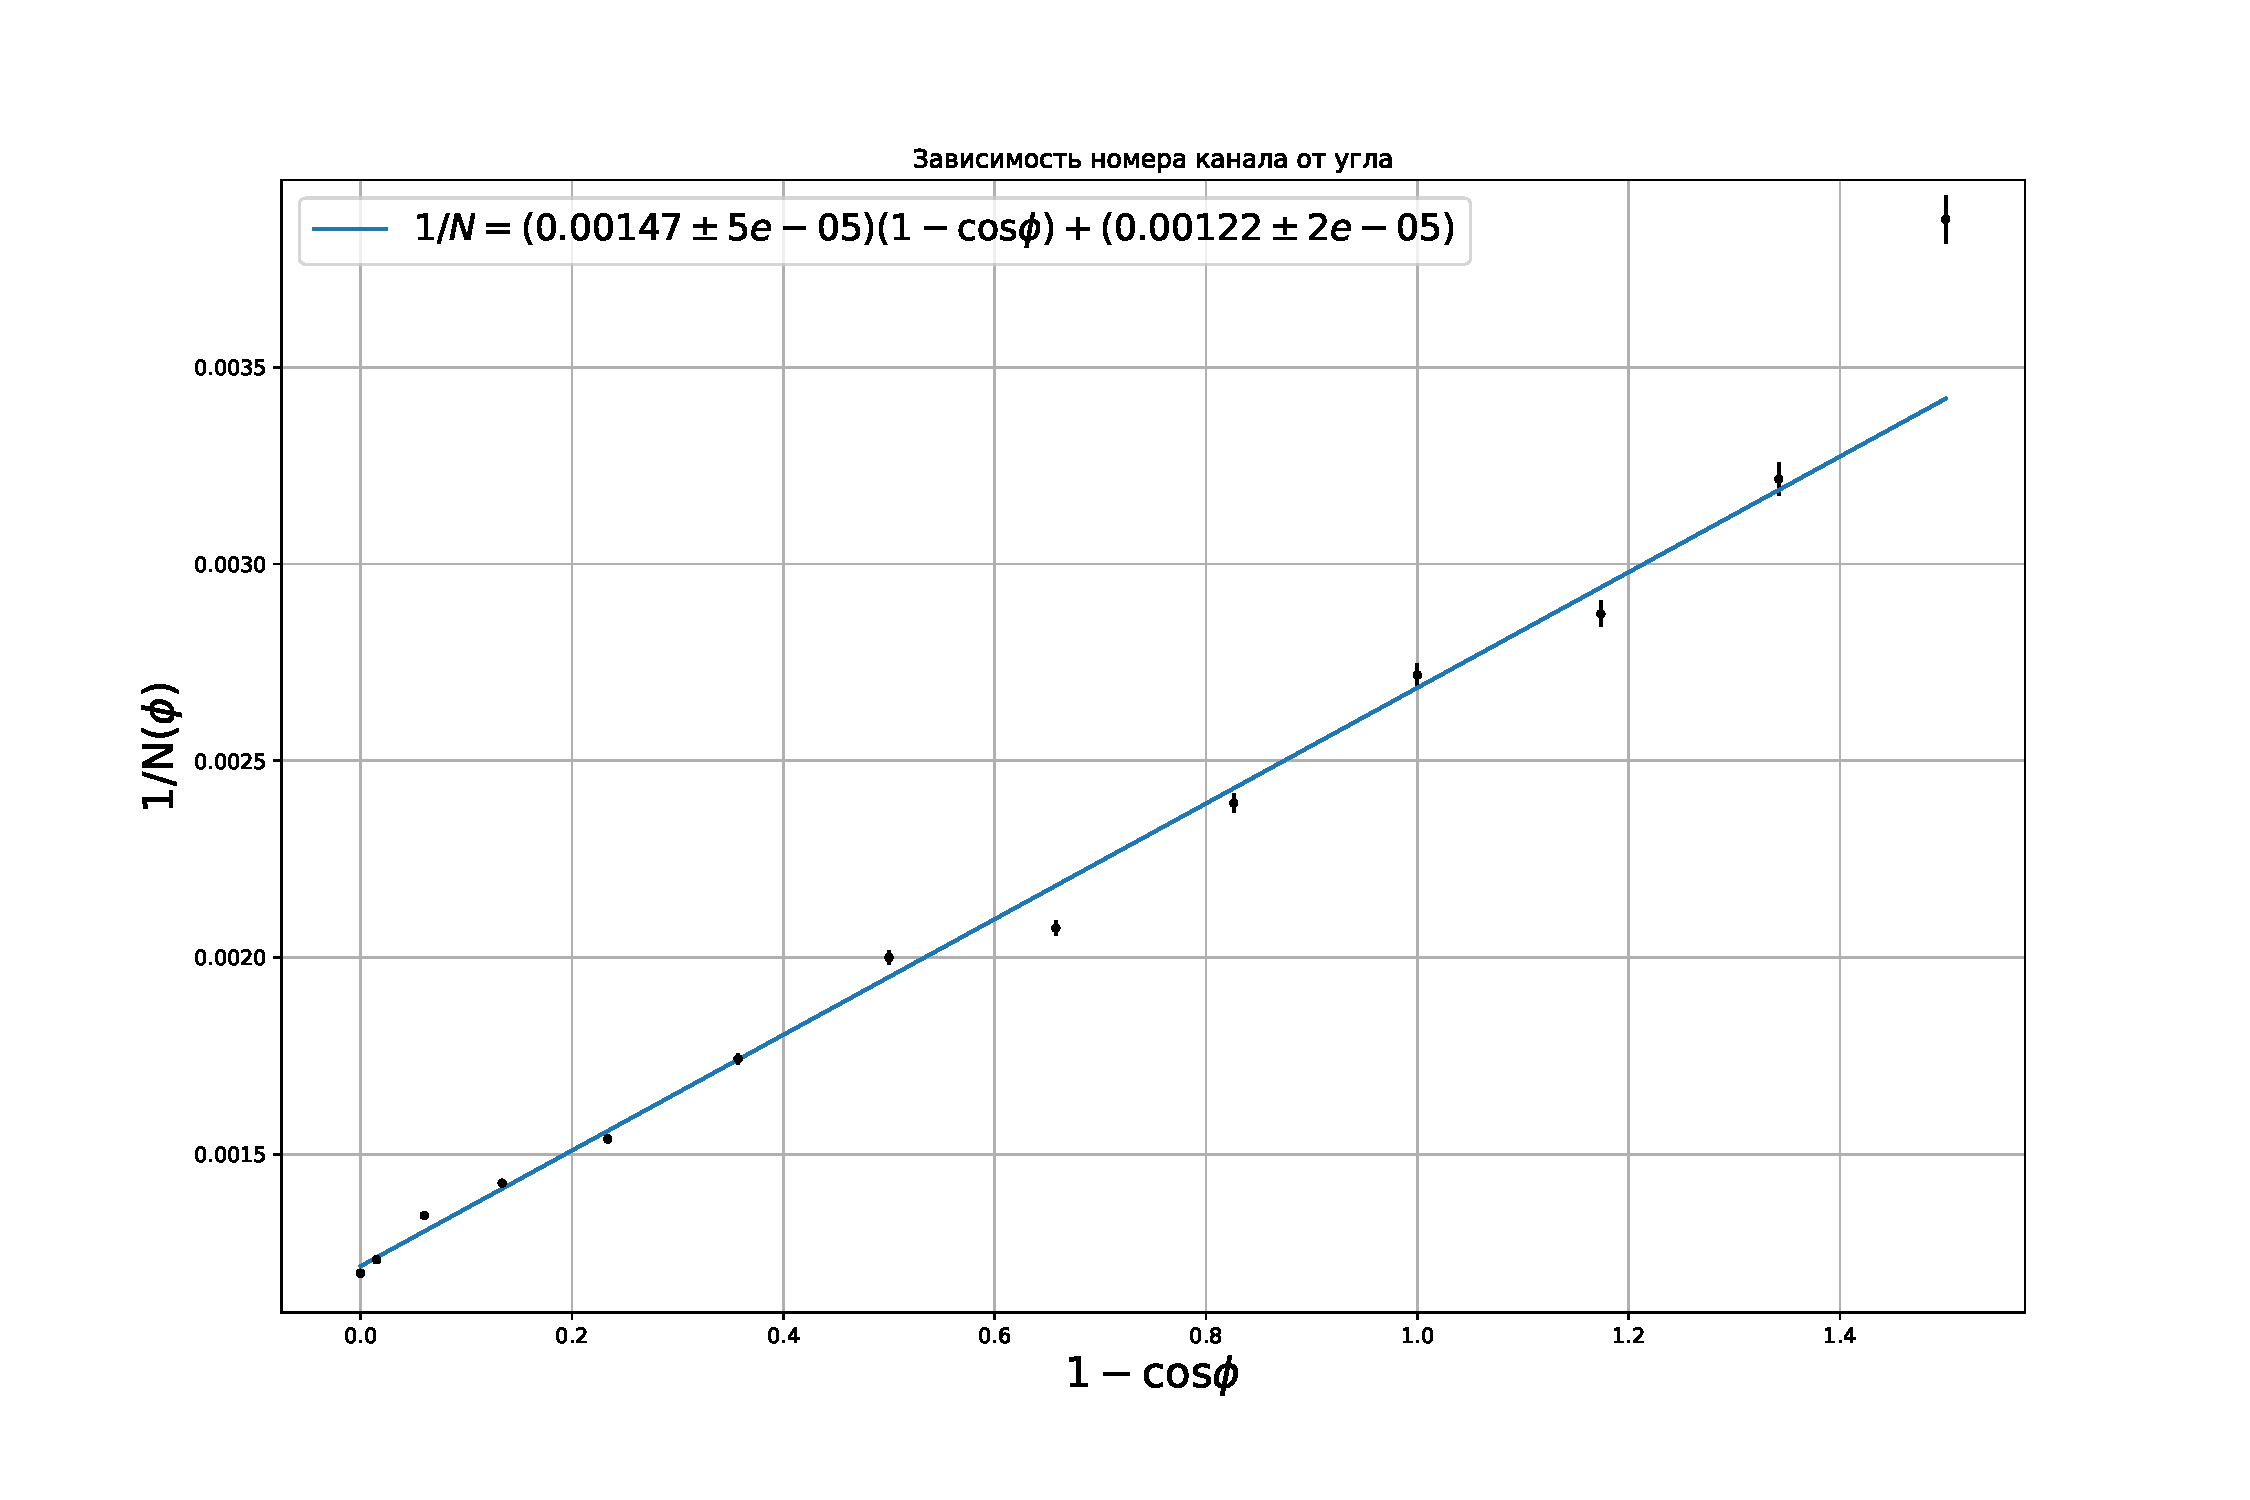
\includegraphics[width=\linewidth]{plot}
        \caption{График зависимости $\dfrac{1}{N(\theta)}= A(1-\cos\theta) + b$}
    \end{figure}
		Погрешности аппроксимации, рассчитанные методом наименьших квадратов: ($y=Ax+b$): $\frac{\sigma A}{A} \approx 0.031$; $\frac{\sigma b}{b} \approx 0.013$.
		
	\item С помощью графика определили коэффициент пропорциональности между N($\theta$) и $\varepsilon(\theta)$: A = $\frac{\varepsilon}{N}\approx 1.47\cdot10^{-3}$.
				
	\item Перейдя от переменной $\varepsilon=\frac{E}{mc^2}$ к энергии E, получаем, что энергия частицы, на которой происходит рассеяние, находится по формуле:
\[ mc^2=E_\gamma\cdot\dfrac{N(90)}{N(0)-N(90)}, \]
	   где $E_\gamma$~---~энергия $\gamma$-лучей, рассеянных источником.
		
		При этом значения  $N(0)$ и $N(90)$ используем полученные из графика (а не полученные непосредственно при измерениях), так как эти значения учитывают измерения, сделанные под другими углами.
\[N_\text{наил.}(0)\approx822.91, \quad N_\text{наил.}(90)\approx372.4, \quad E_{\gamma} = 662\; \K\eV  \]
	Полученная энергия:
\[ E_{\text{эксп.}} = mc^2 = 662 \; \K \eV \cdot \frac{372.4}{822.91-372.4} \approx 547 \; \K \eV \]	
	\item Рассчитаем погрешности измерений:
        \[\dfrac{\sigma N(0)}{N(0)}=\dfrac{\sigma b}{b}\approx0.013 \]
        \[\dfrac{\sigma N(90)}{N(90)}=\sqrt{\left(\frac{\sigma b}{b}\right)^2 + \left(\frac{\sigma A}{A}\right)^2}=\sqrt{(0.031)^2 + (0.013)^2} \approx 0.034 \]
        \[\dfrac{\sigma E}{E}=\sqrt{\left(\frac{\sigma N(90)}{N(90)}\right)^2+\left(\frac{\sigma N(0)+\sigma N(90)}{N(0)-N(90)}\right)^2} = \sqrt{(0.034)^2+\left(\frac{12.63+10.59}{822.91-372.4}\right)^2} \approx 0.062=6.2 \% \]
        
	
	С учётом погрешностей:
	\[ E_{\text{эксп.}} = 547 \pm 34 \; \K \eV \]
	Энергия покоя электрона:
	\[ E_{\text{электр.}}=mc^2=9.1\cdot 10^{-31}\cdot (3\cdot 10^8)^2 \approx 511 \; \K \eV\]
	\end{enumerate}

\section*{Вывод}

Исследовали энергетический спектр $\gamma$-квантов, рассеянных на графите.  Используя полученные данные, построили график зависимости $\frac{1}{N(\theta)}$ от $(1-\cos\theta)$, где N - номер канала в анализаторе, $\theta$ - угол рассеяния. Полученная зависимость оказалась линейная (в пределах погрещности). С её помощью определили энергию покоя частицы, на которой происходит рассеяние: $E_{\text{эксп.}}=547\pm34 \; \K \eV$. В пределах погрешностей полученная величина оказалась близкой к энергии покоя электрона: $E_{\text{электр.}}\approx511 \; \K \eV$, то есть, как и предполагалось, рассеяние происходит на электронах. Погрешность вычисления энергии составила $6.2\%$.
	

\end{document}